\documentclass[landscape]{article}
\usepackage[a4paper,margin=3mm,landscape]{geometry}
\usepackage[scaled=0.92]{helvet}
\usepackage{multicol, multirow}
\usepackage{makecell}
\usepackage{array} 
\usepackage[table]{xcolor}
\usepackage{enumitem} 
\usepackage{amssymb}
\usepackage{graphicx}
\setlist{nosep}

\graphicspath{{./images/}}

\pdfinfo{
    /Title (GEA1000 Cheatsheet.pdf)
    /Creator (TeX)
    /Producer (pdfTeX 1.40.0)
    /Author (Selwyn Ang)
    /Subject (GEA1000)
    /Keywords (GEA1000, Cheatsheet, NUS, Quantitative Reasoning with Data) 
}

% Turn off header and footer
\pagestyle{empty}


\makeatletter
\DeclareRobustCommand\smaller{\@setfontsize\smaller{6pt}{6.5pt}}
\makeatother

% redefine section commands to use less space
\makeatletter
\renewcommand{\section}{\@startsection{section}{1}{0mm}%
  {-0.1ex plus -0.1ex minus -0.1ex}%
  {0.1ex plus .1ex minus 0.1ex}%
{\normalfont\small\bfseries}}
\renewcommand{\subsection}{\@startsection{subsection}{2}{0mm}%
  {-0.1ex plus -0.1ex minus -0.1ex}%
  {0.1ex plus .1ex minus 0.1ex}%
{\normalfont\scriptsize\bfseries}}
\renewcommand{\subsubsection}{\@startsection{subsubsection}{3}{0mm}%
  {-0.1ex plus -0.1ex minus -0.1ex}%
  {0.1ex plus .1ex minus 0.1ex}%
{\normalfont\smaller\bfseries}}%
\makeatother



\renewcommand{\familydefault}{\sfdefault}
\renewcommand\rmdefault{\sfdefault}
%  makes nested numbering (e.g. 1.1.1, 1.1.2, etc)
\renewcommand{\labelenumii}{\theenumii}
\renewcommand{\theenumii}{\theenumi.\arabic{enumii}.}
\renewcommand\labelitemii{•}
\renewcommand\labelitemiii{•}

\setlength{\parindent}{0pt}
\setlength{\parskip}{0pt plus 0.5ex}
\setlength{\columnsep}{0.2cm}
%% adjust spacing for all itemize/enumerate
\setlength{\leftmargini}{0.5cm}
\setlength{\leftmarginii}{0.5cm}
\setlist[itemize,1]{leftmargin=2mm,labelindent=1mm,labelsep=1mm}
\setlist[itemize,2]{leftmargin=2mm,labelindent=1mm,labelsep=1mm}
\setlist[itemize,3]{leftmargin=2mm,labelindent=1mm,labelsep=1mm}
\setlist[enumerate,1]{leftmargin=2mm,labelindent=1mm,labelsep=1mm}
\setlist[enumerate,2]{leftmargin=2mm,labelindent=1mm,labelsep=1mm}
\setlist[enumerate,3]{leftmargin=2mm,labelindent=1mm,labelsep=1mm}

% tightcenter
\newenvironment{tightcenter}{%
  \setlength\topsep{0pt}
  \setlength\parskip{0pt}
  \begin{center}
    }{%
  \end{center}
}

% boxed
\newenvironment{tightbox}{%
  \setlength\topsep{0pt}
  \setlength\parskip{0pt}
  \begin{center}
    \begin{tabular}{|@{\hspace{\dimexpr\fboxsep+0.5\arrayrulewidth}}c@{\hspace{\dimexpr\fboxsep+0.5\arrayrulewidth}}|}
      \hline
    }
    {%
    \\ \hline
    \end{tabular}
  \end{center}
}

% fixed width box
\newenvironment{fixedbox}[1][0.7]{
  \setlength\topsep{0pt}
  \setlength\parskip{0pt}
  \begin{center}
    \begin{tabular}{|>{\centering\arraybackslash}m{#1\linewidth}|}
    \hline
  }{
  \\ \hline
  \end{tabular}
  \end{center}
}

% definition of a new term
\usepackage{soul}
\definecolor{paleyellow}{RGB}{251,243,218}
\newcommand{\definition}[2][]{\sethlcolor{paleyellow}\hl{\textbf{#2}} #1  $\rightarrow$}
% inline definition
\newcommand{\ildefinition}[1]{\sethlcolor{paleyellow}\hl{\textbf{#1}}}

% important note (attention)
\newcommand{\attention}{{\color{red}\textbf{! }}}

% nice proof
\newenvironment{niceproof}[1][Proof]
{%
  \sbox0{\textit{#1}. }%
  \list{}{\labelwidth\wd0 \leftmargin\wd0 \labelsep 0pt }
\item[\usebox0]}
  {\endlist}


\usepackage{color, soul}
\usepackage{listings}
\usepackage{inconsolata}

\definecolor{codegreen}{rgb}{0,0.6,0}
\definecolor{codegray}{rgb}{0.5,0.5,0.5}
\definecolor{codepurple}{HTML}{C42043}
\definecolor{backcolour}{HTML}{F2F2F2}
\definecolor{bookColor}{cmyk}{0,0,0,0.90}

\newcommand{\code}[1]{\texttt{\sethlcolor{backcolour}\hl{$\,$#1$\,$}}}

% SQL code blocks
% define SQL styles
\lstdefinestyle{mySQL}{%
  language=SQL,
  backgroundcolor=\color{backcolour},
  commentstyle=\color{codegreen},
  keywordstyle=\color{codepurple},
  numberstyle=\numberstyle,
  stringstyle=\color{codepurple},
  basicstyle=\scriptsize\ttfamily,
  breaklines=true,
}



% --------------------------------------------------------

\begin{document}
\raggedright
\tiny
\begin{multicols*}{5}
    \setlength{\columnseprule}{0.25pt}

    \begin{tightcenter}
        \fbox{%
          \parbox{0.8\linewidth}{\centering \textcolor{black}{
              {\Large\textbf{GEA1000}}
            \\ \normalsize{AY24/25 SEM 1}}
            \\ {\footnotesize \textcolor{gray}{github/SelwynAng}}
          }%
        }
    \end{tightcenter}
    
    \section{Getting Data}

    \subsection{Exploratory Data Analysis}

      \begin{itemize}
        \item \textbf{Population:} Entire group (of individuals or objects) that we wish to know something about.
        \item \textbf{Research Question:} Seeks to investigate some characteristic of a population.
        \begin{enumerate}
          \item To make an estimate about the population
          \item To test a claim about the population
          \item To compare 2 subpopulations, to investigate a relationship between 2 variables in the population
        \end{enumerate}
        \item \textbf{Exploratory Data Analysis:} Systematic process where we explore a data set and its variables and come up with summary statistics as well as plots
        \begin{enumerate}
          \item Generate research questions about the data
          \item Search for answers to research questions using data visualization tools $\rightarrow$ Can perform data modelling too.
          \item Ask ourselves to what extent does the data we have, answer the questions we are interested in
          \item Refine our existing questions or generate new questions about the data before going back to the data for further exploration
        \end{enumerate}
      \end{itemize}
    
    \subsection{Sampling}
      \begin{itemize}
        \item \textbf{Population of Interest:} Group in which we have interest in drawing conclusions on in a study
        \item \textbf{Population Parameter:} Numerical fact about a population (Eg. Average height \textit{(population parameter)} of all P6 students in a particular primary school \textit{(population)}.)
        \item \textbf{Census:} An attempt to reach out the entire population of interest (However, it has a high cost, takes a long time to complete, may not be able to achieve 100\% response rate)
        \item \textbf{Sample:} Proportion of population selected in the study
        \item \textbf{Estimate:} Inference about the population parameter based on the information obtained from a sample
        \item \textbf{Sampling Frame:} List from which sample was obtained
        \item \textbf{Generalizability:} Ability to generalize findings from a sample to the population
        \begin{enumerate}
          \item Sampling frame must be equal or greater than the population of interest
          \item Probability-based sampling to minimize selection bias
          \item Large sample size to reduce variability or random errors in sample
          \item Minimize non-response rate
        \end{enumerate}
        \item \textbf{Selection bias:} Associated with the researcher's biased selection of units into the sample, caused by imperfect sampling frame or non-probability sampling
        \item \textbf{Non-response bias:} Associated with participants' non-disclosure or non-participation in the research study $\rightarrow$ Exclusion of information from this group (Non-response bias may occur regardless of whether sampling method is probabilistic or non-probabilistic in nature \& can happen in census too)
        \item \textbf{Probability Sampling:} Sampling scheme such that the selection process is done via a known randomized mechanism (Every unit in the sampling frame has a known non-zero probability of being selected, but the probability of being selected does not have to be the same for all units)
        \begin{enumerate}
          \item \underline{Simple Random Sampling (SRS):} Every set of $n$ units has an equal chance to be the sample actually selected
          \item \underline{Systematic Sampling:} Selecting units from a list by applying a selection interval $k$ \& a random starting point from the 1st interval
          \begin{itemize}
            \item Simpler sampling process than SRS as we do not need to know how many sampling units there are exactly
            \item If listing is not random, but instead contains some inherent grouping/ordering of units $\rightarrow$ Possible that a sample produced by systematic sampling may not be representative of population (Sample could have selection bias)
          \end{itemize}
          \item \underline{Stratified Sampling:} Sampling frame is divided into groups called strata, each stratum is similar in characteristics, but size of each stratum does not need to be the same $\rightarrow$ Apply SRS to each stratum (Eg. Taking a SRS of the voters at each polling station (stratum) and then computing the weighted average of the overall vote count, based on size of each stratum)
          \item \underline{Cluster Sampling:} Sampling frame is divided into clusters $\rightarrow$ Fixed number of clusters are then selected using SRS $\rightarrow$ All units from selected clusters are then included in the overall sample 
        \end{enumerate}
        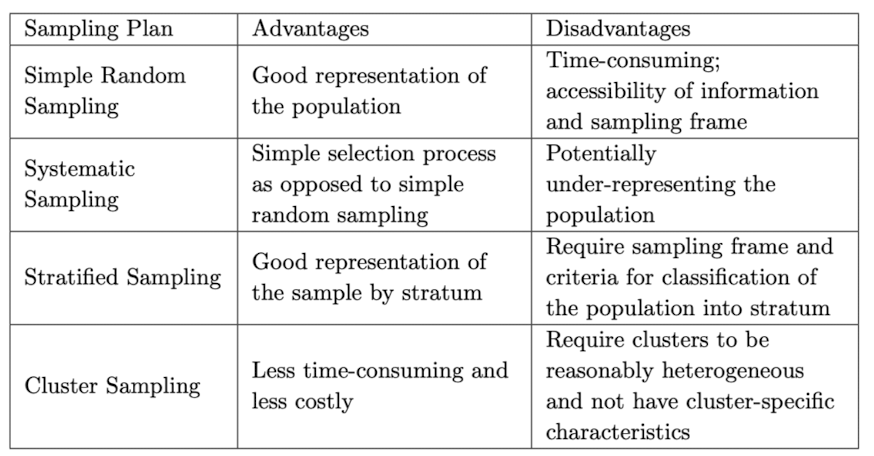
\includegraphics[width=0.9\linewidth]{1_Probability_Sampling.png}
        \item \textbf{Non-probability Sampling:} Selection of units is not done by randomization
        \begin{enumerate}
          \item \underline{Convenience Sampling:} Researcher chooses subjects to form a sample among those that are most easily available to participate in the study (can introduce selection bias \& non-response bias)
          \item \underline{Volunteer Sampling:} Subjects volunteer themselves into a sample (Sample contains subjects who have strong opinion on research question than rest of population)
        \end{enumerate}
      \end{itemize}

    \subsection{Variables and Summary Statistics}
      \begin{itemize}
        \item \textbf{Variable:} Attribute that can be measured or labelled
        \begin{itemize}
          \item \underline{Independent Variable}: Variable subjected to manipulation in a study
          \item \underline{Dependent Variable}: Variable hypothesized to change depending on how the independent variable is manipulated in the study (Does not mean the dependent variable must change)
        \end{itemize}
        \item \textbf{Data Set:} Collection of individuals and variables pertaining to the individuals
        \item \textbf{Categorical Variable:} Variable that take on categories or label values, which are mutually exclusive
        \begin{itemize}
          \item \underline{Ordinal Variable:} Some natural ordering and numbers can be used to represent the ordering
          \item \underline{Nominal Variable:} No intrinsic ordering
        \end{itemize}
        \item \textbf{Numerical Variable:} Variable that take on numerical values, can perform arithmetic operations
        \begin{itemize}
          \item \underline{Discrete Numerical Variable:} There are gaps in the set of possible numbers taken on by the variable
          \item \underline{Continuous Numerical Variable:}  Can take on all possible numerical values in a given range or interval
        \end{itemize}
      \end{itemize}

    \subsection{Summary Statistics - Mean}
      \begin{itemize}
        \item \textbf{Mean:} Average value of a numerical value $x$ ($\overline{x}$)
        \item \textbf{Properties of Mean:}
        \begin{enumerate}
          \item Adding a constant value $c$ to all data points changes the mean by that constant value
          \item Multiplying a constant value of $c$ to all data points will result in the mean being changed by same factor of $c$
          \item Mean does not tell us the distribution of the data
          \item Overall mean can be computed using the weighted average of 2 subgroup means (Eg. Group $A$ has $X$ subjects \& $I$ mean, Group $B$ has $Y$ subjects \& $J$ mean $\rightarrow$ Overall Mean $= \frac{X}{X+Y} * I + \frac{Y}{X+Y} * J$)
          \item Overall mean will always be between the smallest \& largest means among all the subgroups
        \end{enumerate}
      \end{itemize}

    \subsection{Summary Statistics - Variance and Standard Deviation}
      \begin{itemize}
        \item \textbf{Sample Variance, $Var$} = $\frac{(x_1 - \overline{x})^2 + ... + (x_n - \overline{x})^2}{n-1}$
        \item \textbf{Standard Deviation, $S_x$} = $\sqrt{var}$
        \item \textbf{Properties of Standard Deviation:}
        \begin{enumerate}
          \item $s_x$ is always non-negative, when $s_x = 0$: all data points are identical
          \item Adding a constant $c$ to all data points does not change the standard deviation
          \item Multiplying all the data points by a constant $c$ results in the standard deviation being multiplied by $|c|$
          \item Even though mean is $X$ and standard deviation is $Y$, it does not imply that the largest value is $X+Y$
        \end{enumerate}
        \item \textbf{Coefficient of Variation:} Quantifies the degree of spread relative to the mean ($\frac{s_x}{\overline{x}}$)
      \end{itemize}

    \subsection{Summary Statistics - Median, Quartiles, IQR, Mode}
      \begin{itemize}
        \item \textbf{Median:} Middle value of the variable after arranging the values of the data set in ascending or descending order (if there are 2 middle values, we take the average of the 2 middle values as the median)
        \item \textbf{Properties of Median:}
        \begin{enumerate}
          \item When constant $c$ is added to every data point in a data set, median increases by $c$ too
          \item When constant $c$ is multiplied to all data points, median is multiplied by $c$ too
          \item Even when there more than 2 subgroups, overall median will always be between the lowest median and highest median among all the subgroups
        \end{enumerate}
        \item \textbf{Percentiles:} Median is 50th percentile, $Q_1$ is 25th percentile, $Q_3$ is 75th percentile
        \begin{itemize}
          \item Divide data set into lower half \& upper half $\rightarrow$ 1st quartile is median of lower half, 3rd quartile is median of upper half
          \item When data set has odd number of data points, we do not include the median in both the lower and upper halves
        \end{itemize}
        \item \textbf{IQR:} $Q_3 - Q_1$
        \item \textbf{Properties of IQR:}
        \begin{enumerate}
          \item IQR is always non-negative
          \item Adding constant $c$ to all data points results in no change in IQR
          \item Multiplying all data points by a constant $c$ results in IQR being multiplied by $|c|$
        \end{enumerate}
        \item \textbf{Mode:} Numerical value that appears the most often in the data for numerical variable, category that has the highest occurrence in the data for categorical variable
      \end{itemize}
    
    \subsection{Study Designs}
    \begin{itemize}
      \item \textbf{Experimental Study:} Intentionally manipulate 1 variable to observe whether it has an effect on another variable (provide evidence for a cause and effect relationship)
      \begin{itemize}
        \item To establish cause-and-effect relationship between 2 variables, we need to make sure that the independent variable is the only factor that impacts the dependent variable
        \item Random assignment is impartial procedure that uses chance to allocate subjects into treatment \& control groups
        \item If the number of subjects is large, by law of probability, the subjects in the treatment \& control groups will tend to be similar in all aspects
        \item If we make it known to the control group that they are indeed the control group, this could lead to bias
        \item \underline{Placebo:} Inactive substance or other intervention that looks the same as, and is given the same way as, an active drug or treatment being tested (given to control group)
        \item \underline{Single Blinding:} Subjects do not know which group they belong to
        \item \underline{Double Blinding:} Subjects \& assessors are blinded about the assignment
      \end{itemize}
      \item \textbf{Observational Study:} Observes individuals and measures the variables of interest, usually without any direct/deliberate manipulation of the variables by the researchers (do not provide convincing evidence of a cause-and-effect relationship between 2 variables, normally used to circumvent ethical issues in experimental studies)
    \end{itemize}
    
    \section{Categorical Data Analysis}

    \subsection{Rates}
    \begin{itemize}
      \item \textbf{Analyzing 2 categorical variables using a table:} By convention, dependent variable is placed on the columns of the table, while independent variable is placed on the rows
      \item \textbf{Types of Rates:}
      \begin{enumerate}
        \item \underline{Marginal:} Eg. $r(A)$ (relates to 1 categorical variable each time)
        \item \underline{Conditional:} Eg. $r(A|B)$ (set a condition)
        \item \underline{Joint:} Eg. $r(A \& B)$ (total is the baseline)
      \end{enumerate}
    \end{itemize}

    \subsection{Association}
    \begin{itemize}
      \item \textbf{Types of Association:}
      \begin{enumerate}
        \item $rate(A|B) = rate(A|NB)$ : Rate of A is not affected by presence or absence of B
        \item $rate(A|B) > rate(A|NB)$ : Positive association between A and B (Presence of A when B is present is stronger compared to when B is absent)
        \item $rate(A|B) < rate(A|NB)$ : Negative association between A and B (Presence of A when B is present is weaker compared to when B is absent) 
      \end{enumerate}
      \item \textbf{More associations:}
      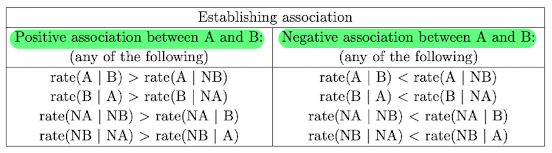
\includegraphics[width=0.9\linewidth]{2_More_associations.png}
    \end{itemize}
    
    \subsection{Rules on Rates}
    \begin{itemize}
      \item \textbf{Symmetry Rules on Rates:}
      \begin{enumerate}
        \item \underline{Symmetry Rule Part 1:} $rate(A|B) > rate(A|NB) \leftrightarrow rate(B|A) > rate(B|NA)$
        \item \underline{Symmetry Rule Part 2:} $rate(A|B) < rate(A|NB) \leftrightarrow rate(B|A) < rate(B|NA)$
        \item \underline{Symmetry Rule Part 3:} $rate(A|B) = rate(A|NB) \leftrightarrow rate(B|A) = rate(B|NA)$
      \end{enumerate}
      \item \textbf{Basic rule on rates:}
      \begin{enumerate}
        \item \underline{Basic rule on rates:} Overall $rate(A)$ will always lie between $rate(A|B)$ and $rate(A|NB)$
        \item \underline{Consequence 1:} Closer $rate(B)$ is to 100\% $\rightarrow$ closer $rate(A)$ is to $rate(A|B)$
        \item \underline{Consequence 2:} $rate(B)$ = 50\% $\rightarrow$ $rate(A) = 0.5(rate(A|B) + rate(A|NB))$
        \item \underline{Consequence 3:} $rate(A|B) = rate(A|NB) \rightarrow rate(A) = rate(A|B) = rate(A|NB)$ 
      \end{enumerate}
    \end{itemize}

    \subsection{Simpson Paradox}
    \begin{itemize}
      \item \textbf{Definition:} Phenomenon in which a trend appears in more than half of the groups of data but disappears (variables are no longer associated) or reverses when the groups are combined
      \item \underline{Note:} In examples where there more than 2 subgroups, Simpson Paradox is observed as long as a majority of individual subgroup rates show the opposite trend to the overall rate
      \item \textbf{Relationship between SP \& Confounding variables:} 
      \begin{enumerate}
        \item When Simpson Paradox is observed $\rightarrow$ There is definitely a confounding variable present (3rd variable that is associated with the 2 variables whose relationship we are investigating)
        \item Existence of confounder $\nRightarrow$ Observation of Simpson Paradox
      \end{enumerate}
    \end{itemize}

    \subsection{Confounders}
    \begin{itemize}
      \item \textbf{Definition:} Confounder is a 3rd variable that is associated with both the independent and dependent variables whose relationship we are investigating
      \item \underline{Note:} A confounding variable is associated with both independent \& dependent variables, so removing 1 of the associations is enough to remove the confounding variable
      \item An alternative approach to address potential confounders is to rely on random assignment (However, random assignment is not possible all the time)
      \item Only slicing can be done to control for confounder in Observational studies. Random assignment is only suitable for Experimental studies.

    \end{itemize}

    \section{Dealing with Numerical Data}

    \subsection{Univariate Exploratory Data Analysis}
    \begin{itemize}
      \item \textbf{Distribution:} An orientation of data points, broken down by their observed number or frequency of occurrence
      \item \textbf{Histograms:} A histogram is a graphical representation that organizes data points into ranges or bins (Left-end point of interval is excluded, aka. $bin\_interval = (a,b]$)
      \begin{enumerate}
        \item Unimodal (1 distinct peak)
        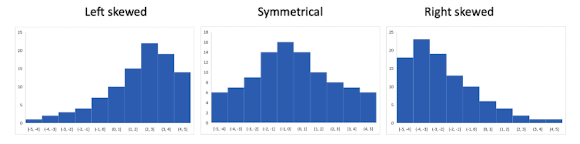
\includegraphics[width=0.9\linewidth]{3_skewed.png}
        \item Bimodal (2 distinct peaks)
        \item Multimodal (more than 1 distinct peaks)
      \end{enumerate}
      \item \textbf{Note about histograms:} Histogram shows distribution of numerical variable across a number line, while bar graphs show different categories of categorical variable
      \item \textbf{Symmetrical Distribution - Bell Curve:} Normal Distribution
      \item \textbf{Central Tendency - Mean, Median, Mode}:
      \begin{itemize}
        \item \underline{Symmetrical distribution:} Mean, median, mode very close to each other near peak of distribution
        \item \underline{Left skewed distribution:} Usually (but not always) have mean $<$ median $<$ mode
        \item \underline{Right skewed distribution:} Usually (but not always) have mode $<$ median $<$ mean
      \end{itemize}
      \item \textbf{Spread - Standard deviation and range}:
      \begin{itemize}
        \item \underline{Standard Deviation:} Measure of variability around central Tendency
        \item \underline{Range:} Difference between largest and smallest data points in the distribution
      \end{itemize}
      \item \textbf{Outlier:} Observation that falls well above or below overall bulk of the data 
      \begin{itemize}
        \item Outliers should not be removed unnecessarily as they do tell us something about the behavior of the variable and prompt us to investigate further why such extreme values can happen
        \item Mean is most affected by removal of outlier, while median and mode either remains the same or only change slightly (Median and mode are robust statistics)
        \item Data point is considered an outlier if it is greater than $Q_3 + 1.5*IQR$ or less than $Q_1 - 1.5*IQR$
      \end{itemize}
      \item \textbf{Box-plots for Univariate EDA:}
      \begin{itemize}
        \item To construct box-plots, we need the five number summary (Minimum, Q1, Median, Q3, Maximum)
        \item Upper half of data have greater variability than lower half $\rightarrow$ Distribution is right-skewed
      \end{itemize}
      \item \textbf{Histograms VS Box-plots}
      \begin{enumerate}
        \item Histogram gives better sense of shape of distribution of variable, compared to box-plots
        \item To compare distributions of different data sets, putting different box-plots side by side is more illustrative than using histograms
        \item Box-plots do a better job than histograms at identifying and indicating outliers
        \item Number of data points we have in a data set is better shown in a histogram than in a box-plot (2 distributions with very different number of data points can have almost identical box-plots)
      \end{enumerate}
    \end{itemize}

    \subsection{Bivariate Exploratory Data Analysis}
    \begin{itemize}
      \item \textbf{Scatter Plot:} Gives us an idea of the pattern formed by data between 2 variables in question
      \item \textbf{Correlation Coefficient:} Quantifies the level of linear association between 2 variables
      \item \textbf{Direction of Relationship:} Either positive (increase in 1 of the variables is associated with an increase in the other variable), negative (increase in 1 of the variables is associated with decrease in the other) or neither
      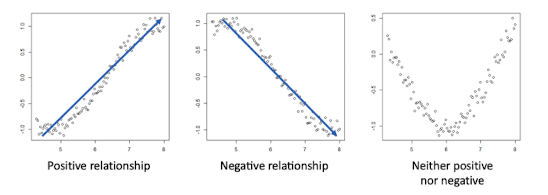
\includegraphics[width=0.9\linewidth]{4_direction.png}
      \item \textbf{Form of Relationship:} Describes general shape of scatter plot (linear or non-linear)
      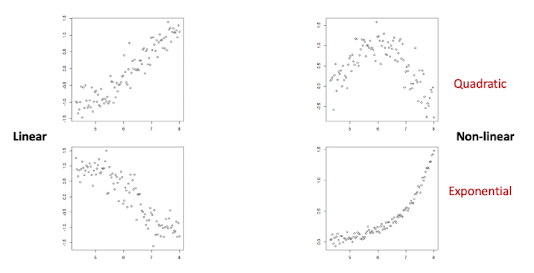
\includegraphics[width=0.9\linewidth]{5_form.png}
      \item \textbf{Strength of Relationship:} Indicates how closely the data follow the form of the relationship
      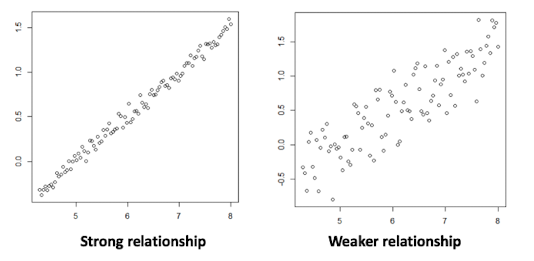
\includegraphics[width=0.9\linewidth]{6_strength.png}
    \end{itemize}

    \subsection{Correlation Coefficient}
    \begin{itemize}
      \item Measures the linear association between 2 variables, denoted by $r$, ranges $[-1, 1]$, summarizes the direction and strength of linear association between 2 variables
      \item $r>0 \rightarrow$ Association is positive, $r<0 \rightarrow$ Association is negative, $r=1$ or $r=-1 \rightarrow$ Perfect association, $r=0 \rightarrow$ No linear association 
      \item Magnitude of $r$ tells us the strength of linear association between 2 numerical variables
      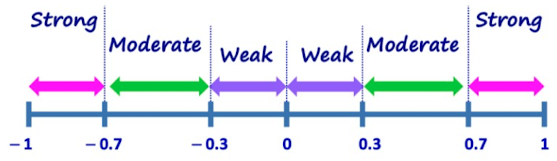
\includegraphics[width=0.9\linewidth]{7_r_values.png}
      \item No linear association between variables does not necessarily mean no association between variables (Eg. Quadratic relationship)
      \item When a straight line joining all data points is actually a straight horizontal or vertical line $\rightarrow r=0$ and there is no association between 2 variables
      \item \underline{Computing Correlation Coefficient (assuming bivariate data $(x,y)$):}
      \begin{enumerate}
        \item Compute mean and standard deviation of $x$ and $y$
        \item Convert each value of $x$ and $y$ into standard units ($\frac{x-\overline{x}}{s_x}$) and ($\frac{y-\overline{y}}{s_y}$)
        \item Compute the product $xy$ in their standard units for each data point
        \item Sum the products $xy$ over all data points, then divide the sum by $n-1$, where $n$ is the number of data points $\rightarrow$ Result is $r$
      \end{enumerate}
      \item $r$ is not affected by interchanging the $x$ and $y$ variables
      \item $r$ is not affected by adding a number to all values of a variable
      \item $r$ is not affected by multiplying a positive number to all values of a variable
      \item Association is not causation (we can only conclude a statistical relationship between x and y, not a causal relationship)
      \item $r$ does not tell us anything about non-linear association
      \item Outliers can affect $r$ significantly
      \item \underline{Fallacies}
      \begin{itemize} 
        \item Ecological correlation is computed based on aggregates rather than on individuals
        \item In general, when association for both individuals and aggregates are in the same direction, ecological correlation based on aggregates will typically overstate the strength of association in individuals
      \end{itemize}
      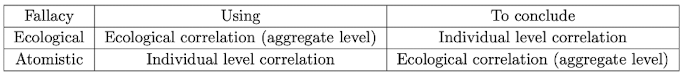
\includegraphics[width=1.0\linewidth]{8_fallacies.png}
    \end{itemize}

    \subsection{Linear Regression}
    \begin{itemize}
      \item \textbf{Equation of straight line:} $y=mX+b$
      \item \textbf{Sum of Squares of Errors:} $e_1^2 + e_2^2 + ... + e_n^2$ where $e_i = y_{pred} - y_{actual}$
      \item \textbf{Notes:}
      \begin{enumerate}
        \item Least squares regression line obtained from a set of observed data points will always pass through $(\overline{x}, \overline{y})$
        \item Regression line to predict $y$ based on $x$ cannot be used to predict $x$ based on $y$
        \item Given $Y=mX+b \rightarrow m = \frac{s_Y}{s_X}r$ 
        \item We should not use the regression line to make prediction outside the independent variable's range in the data set
        \item \underline{Transform into linear relationship:} $y=cb^t == ln(y) = ln(c) + tln(b)$
      \end{enumerate}
    \end{itemize}
    
    \section{Statistical Inference}
    \subsection{Probability}
    \begin{itemize}
      \item \textbf{Sample Space:} Collection of all possible outcomes of a probability experiment
      \item \textbf{Event:} Sub-collection of the sample space
      \item \textbf{Rules of Probability:}
      \begin{enumerate}
        \item $P(E)$ is a number between 0 and 1
        \item $P(S)$ is 1
        \item If $E$ and $F$ are mutually exclusive events $\rightarrow P(E \cup F) = P(E) + P(F)$
      \end{enumerate}
      \item \textbf{Uniform Probability:} Way of assigning probabilities to outcomes such that equal probability is assigned to every outcome in the finite sample space
    \end{itemize}

    \subsection{Conditional Probability and Independence}
    \begin{itemize}
      \item \textbf{Conditional Probability:} $P(E|F) = \frac{P(E \cap F)}{P(F)}$
      \item \textbf{Prosecutor Fallacy:} Mistake of confusing $P(A|B)$ as $P(B|A)$ (Unless $P(A)$ == $P(B)$)
      \item \textbf{Independence:} $A$ and $B$ are independent $\rightarrow P(A) = P(A|B) == P(A) * P(B) = P(A \cap B)$ ($A$ and $B$ are independent events whenever $A$ and $B$ are not associated with each other)
      \item \textbf{Conditionally Independence:} $A$ and $B$ are conditionally independent given an event $C$ if $P(A \cap B|C) = P(A|C) * P(B|C)$
    \end{itemize}
    
    \subsubsection{Conjunction Fallacy, Base Rate Fallacy, Random Variables}
    \begin{itemize}
      \item \textbf{Law of Total Probability:} If $E$, $F$, $G$ are events from the same sample space $S$ such that (1): $E$ and $F$ are mutually exclusive and (2): $E \cup F = S \rightarrow P(G) = P(G|E) * P(E) + P(G|F) * P(F)$ 
      \item \textbf{Conjunction Fallacy:} One would have committed Conjunction Fallacy if one believes that $P(A \cap B) > P(A)$ or $P(A \cap B) > P(B)$ (Chances of 2 things happening together is higher than the chance of 1 of those things happening alone) $\rightarrow$ What is actually true is $P(A \cap B) \leq P(A)$ and $P(A \cap B) \leq P(B)$
      \item \textbf{Base Rate Fallacy:} A decision-making error in which information about the rate of occurrence of some trait in a population, called the base rate information, is ignored or not given appropriate weight
      \item \textbf{True Positive Rate:} $P(Test Positive | Individual Is Infected)$ (Sensitivity of test)
      \item \textbf{True Negative Rate:} $P(Test Negative | Individual Is Not Infected)$ (Specificity of test)
      \item \textbf{Random Variable:} Numerical variable with probabilities assigned to each of the possible numerical values taken by the numerical variable
      \begin{enumerate}
        \item Discrete random variable
        \item Continuous random variable
      \end{enumerate}
    \end{itemize}

    \subsection{Statistical Inference and Confidence Intervals}
    \begin{itemize}
      \item \textbf{Statistical Inference:} Use of samples to draw inferences or conclusions about the population in question
      \item \textbf{Sample Statistic:} Sample Statistic = Population parameter + bias + random error (By adopting good sampling methods, we can reduce selection bias. Having high response rate will minimize non-response bias)
      \item \textbf{Confidence Interval:} Range of values that is likely to contain a population parameter based on a degree of confidence
      \begin{itemize}
        \item \underline{Confidence Interval for population proportion:} $p^* \pm z^* * \sqrt{\frac{p^*(1-p^*)}{n}}$, where $p^*$ is sample proportion, $z^*$ is z-value from standard normal distribution, $n$ is sample size
        \item \underline{Confidence Interval for population mean:} $\overline{x} \pm t^* * \frac{s}{\sqrt{n}}$, where $\overline{x}$ is sample mean, $t^*$ is "t-value" from t-distribution, $s$ is sample SD, $n$ is sample size 
        \item \underline{Margin of error:} Directly impacts the width of the confidence interval
        \item "95\% confident" means that if many simple random samples of the same size are taken, and a confidence interval is constructed for each of them, then about 95\% of the confidence intervals constructed would contain the population parameter
        \item Either the population parameter is in the interval or is not (Wrong to say there is a 95\% chance that it is in the interval, there is no probabilistic element)
        \item \underline{Properties of Confidence Intervals}
        \begin{enumerate}
          \item Larger the sample size, the smaller the random error $\rightarrow$ Results in a narrower confidence interval
          \item Higher the confidence level at which the confidence interval is constructed $\rightarrow$ Wider the confidence interval
        \end{enumerate}
      \end{itemize}
    \end{itemize}

    \subsection{Hypothesis Testing}
    \begin{itemize}
      \item \textbf{Definition:} Statistical inference method used to decide if the data from a random sample is sufficient to support a particular hypothesis about a population
      \item \textbf{5 steps of hypothesis test:}
      \begin{enumerate}
        \item Identify the questions, state the null hypothesis and alternative hypothesis
        \item Set significance level of test
        \item Using sample, find the relevant sample statistic
        \item With sample statistic and hypothesis, calculate p-value
        \item Make conclusion of hypothesis test (dependent on p-value and significance level of test)
      \end{enumerate}
      \item \textbf{p-value:} Probability of obtaining a result as extreme or more extreme than our observation in the direction of the alternative hypothesis, assuming the null hypothesis is true
      \begin{itemize}
        \item p-value $<$ significance level: Sufficient evidence to reject null hypothesis in favor of the alternative hypothesis
        \item p-value $\geq$ significance level: Insufficient evidence to reject the null hypothesis. The hypothesis test is inconclusive. This does not mean that we accept the null hypothesis
      \end{itemize}
      \item \textbf{Hypothesis test for population proportion/mean:} $H_0$: population parameter = null value, $H_1$: population parameter $<$ null value or $H_1$: population parameter $>$ null value
      \item \textbf{Hypothesis test for association:} $H_0$: No association, $H_1$: There is an association
    \end{itemize}

    \section{End-of-chapter Questions Pointers:}
    \subsection{Chapter 1}
    \begin{itemize}
      \item Control group can simply be not receiving treatment, receiving a placebo, or receiving an existing treatment (with known success rate)
      \item Observational studies generally have control groups (subjects are self-assigned to different treatment \& control groups)
    \end{itemize}

    \subsection{Chapter 2}
    \begin{itemize}
      \item Given $Rate(Male) = 0.4, Rate(Male|MilkTea)=0.6, Rate(Male|FruitTea)=0.3$, $Rate(Male)$ is closer to $Rate(Male|FruitTea) \rightarrow$ Closer $Rate(FruitTea)$ is to 100\%
      \item Since $Rate(Email)=0.45, Rate(Email|Response)=0.5, Rate(Email|Non-response)=0.4$, then $Rate(Response)=0.5$
    \end{itemize}

    \subsection{Chapter 3}
    \begin{itemize}
      \item Associations are not necessarily transitive
      \item Given that correlation coefficients for males and females is positive each, it is possible for correlation coefficient for both combined is negative
      \item Predicted value based on regression line is NOT equal to actual/exact value
    \end{itemize}

    \subsection{Chapter 4}
    \begin{itemize}
      \item By the interpretation of confidence intervals via repeated sampling, we conclude that about 95\% of the samples will contain the population parameter within their respective confidence intervals.
      \item Any confidence interval constructed from any sample, regardless of the significance level, may or may not contain the population parameter
      \item Hypothesis tests regarding statements about the population should be conducted on probability-based samples only (not census)
    \end{itemize}
\end{multicols*}
\end{document}
